\documentclass[conference]{IEEEtran}
\IEEEoverridecommandlockouts
% The preceding line is only needed to identify funding in the first footnote. If that is unneeded, please comment it out.
\usepackage{cite}
\usepackage{amsmath,amssymb,amsfonts}
\usepackage{ngerman}
\usepackage{algorithmic}
\usepackage{graphicx}
\usepackage{textcomp}
\usepackage{xcolor}
\usepackage{tikz}
\def\BibTeX{{\rm B\kern-.05em{\sc i\kern-.025em b}\kern-.08em
    T\kern-.1667em\lower.7ex\hbox{E}\kern-.125emX}}
\begin{document}

\title{Conference Paper Title*\\
{\footnotesize \textsuperscript{*}Note: Sub-titles are not captured in Xplore and
should not be used}
\thanks{Identify applicable funding agency here. If none, delete this.}
}

\author{
\IEEEauthorblockN{1\textsuperscript{st} Karina Heins}
\IEEEauthorblockA{\textit{DHBW Ravensburg Campus Friedrichshafen} \\
\textit{Mercedes-Benz AG}\\
Friedrichshafen,  Germany \\
heins.karina-tfe18@it.dhbw-ravensburg.de}
\and
\IEEEauthorblockN{2\textsuperscript{st} Florian Schatz}
\IEEEauthorblockA{\textit{DHBW Ravensburg Campus Friedrichshafen} \\
\textit{Mercedes-Benz AG}\\
Friedrichshafen,  Germany \\
schatz.florian-tfe18@it.dhbw-ravensburg.de}
\and
\IEEEauthorblockN{3\textsuperscript{st} Patrick Madlindl}
\IEEEauthorblockA{\textit{DHBW Ravensburg Campus Friedrichshafen} \\
\textit{Mercedes-Benz AG}\\
Friedrichshafen,  Germany \\
madlindl.patri-tfe18@it.dhbw-ravensburg.de}
\and
\IEEEauthorblockN{4\textsuperscript{st} Marcel Dirschinger}
\IEEEauthorblockA{\textit{DHBW Ravensburg Campus Friedrichshafen} \\
\textit{Airbus Helicopters AG}\\
Friedrichshafen,  Germany \\
dirschinger.marcel-tfe18@it.dhbw-ravensburg.de}
}

\maketitle

\begin{abstract}
This document is a model and instructions for \LaTeX.
This and the IEEEtran.cls file define the components of your paper [title, text, heads, etc.]. *CRITICAL: Do Not Use Symbols, Special Characters, Footnotes, 
or Math in Paper Title or Abstract.
\end{abstract}

\begin{IEEEkeywords}
component, formatting, style, styling, insert
\end{IEEEkeywords}

\section{Einleitung}
Sowohl in der Informatik als auch in anderen Bereichen müssen häufig Daten nach bestimmten Attributen sortiert werden. Liegen diese in digitaler Form vor, kann eine Sortierung der Daten über Sortieralgorithmen gelöst werden. Bei kleinen Datensätzen ist die Wahl des Sortieralgorithmus aufgrund der geringen Laufzeit nahezu irrelevant. Steigt die Datensatzgröße, so verlängert sich die Sortierzeit. Zur Verkürzung dieser können effiziente Sortierverfahren wie Merge-Sort verwendet werden. In der heutigen Zeit ist die Menge der anfallenden Daten, wie Messreihen aus wissenschaftlichen oder technischen Versuchen im Verhältnis zur verfügbaren Rechenleistung eines Computers massiv gestiegen. Daher ist eine effiziente Möglichkeit für Sortierung von hoher Bedeutung. Zur darüber hinausgehenden Laufzeitoptimierung kann Cloud-Computing eingesetzt werden. Hierbei werden Rechenaufgaben nicht auf einem einzelnen Computer ausgeführt, sondern können unter Einsatz von Parallelisierungswerkzeugen wie das Message Passing Interface (MPI) auf mehrere Maschinen (genannt Knoten) verteilt werden. In dieser Arbeit wird am Beispiel der alphabetischen Wörtersortierung untersucht, ob eine Aufteilung der Sortieraufgabe zu einer Senkung der Laufzeit beitragen kann. Hierzu wird der Sortieralgorithmus parallelisiert und in einer Cloud-Umgebung verteilt ausgeführt.
\section{Grundlagen}
\subsection{Merge Sort}
\subsection{Merge Sort}
Merge-Sort ist ein effizienter Algorithmus zur Sortierung vergleichbarer Datenobjekte.  Der Algorithmus setzt sich dem Namen nach aus \glqq merge\grqq{} (engl.  für Verschmelzen) und \glqq sort\grqq{} (engl.  für Sortieren) zusammen und wurde 1945 durch John von Neumann vorgestellt. Es handelt sich um einen stabilen Sortieralgorithmus,  der die Reihenfolge zusammengehöriger Eingangsdaten bei eventueller Sortierung über einen weiteren Parameter nicht manipuliert. Außerdem arbeitet der Algorithmus nach dem \glqq Teile und Hersche\grqq{}-Prinzip und setzt dafür folglich auf Rekursion, Merge-Sort wird zum Sortieren und Arrays/Listen bzw.  anderen listenähnlichen Datenstrukturen verwendet.\\
\begin{figure}[htbp]
\centering
% 5-2-3-1-4    10
% 5-2 3-1-4	8.5
% 5 2 3 1-4	7
% 5 2 3 1 4	5.5
% 2-5 3 1-4	4
% 2-5 1-3-4	2.5
%1-2-3-4-5	1
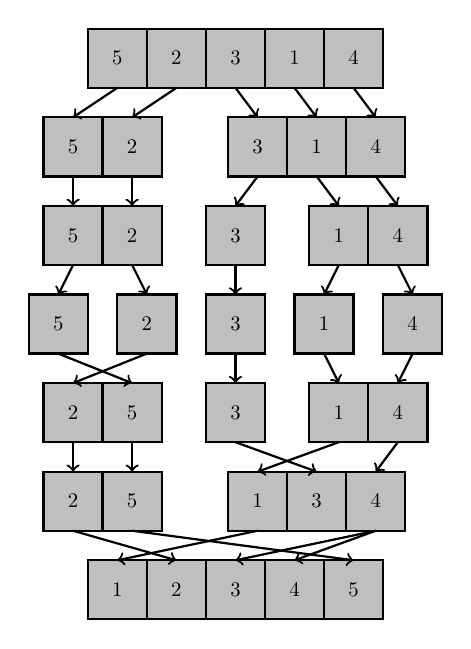
\begin{tikzpicture}[scale=0.75, transform shape]
\draw [thick, fill=gray!50] (1,9) rectangle(2,10) node[pos=.5] {5};
\draw [thick, fill=gray!50] (2,9) rectangle(3,10) node[pos=.5] {2};
\draw [thick, fill=gray!50] (3,9) rectangle(4,10)node[pos=.5] {3};
\draw [thick, fill=gray!50] (4,9) rectangle(5,10)node[pos=.5] {1};
\draw [thick, fill=gray!50] (5,9) rectangle(6,10)node[pos=.5] {4};

\draw [thick, fill=gray!50] (0.25,7.5) rectangle(1.25,8.5)node[pos=.5] {5};
\draw [thick, fill=gray!50] (1.25,7.5) rectangle(2.25,8.5)node[pos=.5] {2};
\draw [thick, fill=gray!50] (3.375,7.5) rectangle(4.375,8.5)node[pos=.5] {3};
\draw [thick, fill=gray!50] (4.375,7.5) rectangle(5.375,8.5)node[pos=.5] {1};
\draw [thick, fill=gray!50] (5.375,7.5) rectangle(6.375,8.5)node[pos=.5] {4};

\draw [thick, fill=gray!50] (0.25,6) rectangle(1.25,7)node[pos=.5] {5};
\draw [thick, fill=gray!50] (1.25,6) rectangle(2.25,7)node[pos=.5] {2};
\draw [thick, fill=gray!50] (3,6) rectangle(4,7)node[pos=.5] {3};
\draw [thick, fill=gray!50] (4.75,6) rectangle(5.75,7)node[pos=.5] {1};
\draw [thick, fill=gray!50] (5.75,6) rectangle(6.75,7)node[pos=.5] {4};

\draw [thick, fill=gray!50] (0,4.5) rectangle(1,5.5)node[pos=.5] {5};
\draw [thick, fill=gray!50] (1.5,4.5) rectangle(2.5,5.5)node[pos=.5] {2};
\draw [thick, fill=gray!50] (3,4.5) rectangle(4,5.5)node[pos=.5] {3};
\draw [thick, fill=gray!50] (4.5,4.5) rectangle(5.5,5.5)node[pos=.5] {1};
\draw [thick, fill=gray!50] (6,4.5) rectangle(7,5.5)node[pos=.5] {4};

\draw [thick, fill=gray!50] (0.25,3) rectangle(1.25,4)node[pos=.5] {2};
\draw [thick, fill=gray!50] (1.25,3) rectangle(2.25,4)node[pos=.5] {5};
\draw [thick, fill=gray!50] (3,3) rectangle(4,4)node[pos=.5] {3};
\draw [thick, fill=gray!50] (4.75,3) rectangle(5.75,4)node[pos=.5] {1};
\draw [thick, fill=gray!50] (5.75,3) rectangle(6.75,4)node[pos=.5] {4};

\draw [thick, fill=gray!50] (0.25,1.5) rectangle(1.25,2.5)node[pos=.5] {2};
\draw [thick, fill=gray!50] (1.25,1.5) rectangle(2.25,2.5)node[pos=.5] {5};
\draw [thick, fill=gray!50] (3.375,1.5) rectangle(4.375,2.5)node[pos=.5] {1};
\draw [thick, fill=gray!50] (4.375,1.5) rectangle(5.375,2.5)node[pos=.5] {3};
\draw [thick, fill=gray!50] (5.375,1.5) rectangle(6.375,2.5)node[pos=.5] {4};

\draw [thick, fill=gray!50] (1,0) rectangle(2,1)node[pos=.5] {1};
\draw [thick, fill=gray!50] (2,0) rectangle(3,1)node[pos=.5] {2};
\draw [thick, fill=gray!50] (3,0) rectangle(4,1)node[pos=.5] {3};
\draw [thick, fill=gray!50] (4,0) rectangle(5,1)node[pos=.5] {4};
\draw [thick, fill=gray!50] (5,0) rectangle(6,1)node[pos=.5] {5};
\draw [thick,draw=black,->] (3.875,1.5) -- (1.5,1);
\draw [thick,draw=black,->] (0.75,1.5) -- (2.5,1);
\draw [thick,draw=black,->] (5.875,1.5) -- (3.5,1);
\draw [thick,draw=black,->] (5.875,1.5) -- (4.5,1);
\draw [thick,draw=black,->] (1.75,1.5) -- (5.5,1);
\draw [thick,draw=black,->] (0.75,3) -- (0.75,2.5);
\draw [thick,draw=black,->] (1.75,3) -- (1.75,2.5);
\draw [thick,draw=black,->] (3.5,3) -- (4.875,2.5);
\draw [thick,draw=black,->] (5.25,3) -- (3.875,2.5);
\draw [thick,draw=black,->] (6.25,3) -- (5.875,2.5);
\draw [thick,draw=black,->] (2,4.5) -- (0.75,4);
\draw [thick,draw=black,->] (0.5,4.5) -- (1.75,4);
\draw [thick,draw=black,->] (3.5,4.5) -- (3.5,4);
\draw [thick,draw=black,->] (5,4.5) -- (5.25,4);
\draw [thick,draw=black,->] (6.5,4.5) -- (6.25,4);
\draw [thick,draw=black,->] (0.75,6) -- (0.5,5.5);
\draw [thick,draw=black,->] (1.75,6) -- (2,5.5);
\draw [thick,draw=black,->] (3.5,6) -- (3.5,5.5);
\draw [thick,draw=black,->] (5.25,6) -- (5,5.5);
\draw [thick,draw=black,->] (6.25,6) -- (6.5,5.5);
\draw [thick,draw=black,->] (0.75,7.5) -- (0.75,7);
\draw [thick,draw=black,->] (1.75,7.5) -- (1.75,7);
\draw [thick,draw=black,->] (3.875,7.5) -- (3.5,7);
\draw [thick,draw=black,->] (4.875,7.5) -- (5.25,7);
\draw [thick,draw=black,->] (5.875,7.5) -- (6.25,7);
\draw [thick,draw=black,->] (1.5,9) -- (0.75,8.5);
\draw [thick,draw=black,->] (2.5,9) -- (1.75,8.5);
\draw [thick,draw=black,->] (3.5,9) -- (3.875,8.5);
\draw [thick,draw=black,->] (4.5,9) -- (4.875,8.5);
\draw [thick,draw=black,->] (5.5,9) -- (5.875,8.5);
\end{tikzpicture}
\caption[Darstellung Merge-Sort Beispiel]{Ablauf eines Merge-Sort über ein Array aus Beispielzahlen}
\label{fig:mergesort}
\end{figure}
Um die Elemente der Datenstruktur (im Folgenden Liste) sortieren zu können,  werden diese zunächst rekursiv geteilt.  Dafür wird die Liste in eine linke und rechte Hälfte geteilt.  Die Hälften stellen jetzt jeweils die Basis für den nächsten Rekursions- bzw- Teilungsschritt dar. Der Vorgang wird wiederholt,  bis pro Teilliste lediglich ein weiters Element vorhanden ist.  Die Teilung der Datenelemente fordert nahezu keine Rechenleistung und benötigt keinen zusätzlichen Speicherplatz.  Im Anschluss wird die Rekursion der Teilung für den eigentlichen Sortiervorgang zurück durchlaufen. Die geteilten Listen werden nun innerhalb der Rekursion zu Zweierpaaren jeweils sortiert in eine neue Liste zusammengeführt. In der Informatik wird dabei auch von Konkatenierung gesprochen.  Aufgrund der Zusammenführung der Listen aus zwei bereits sortierten Teillisten können im Sortiervorgang jeweils die ersten Elemente verglichen werden. Das Element mit dem niedrigeren Wert wird in die Liste der Zusammenführung gespeichert.  Da in diesem Schritt zeitgleich drei Listen vorhanden sind wird hier abseits des ursprünglichen Datenspeichers zusätzlicher Speicher benötigt.  Aufgrund der Vergleiche ergibt sich in der Zusammenführung der überwiegende Rechenaufwand des Algorithmus.  Der Ablauf des \glqq merge\grqq{} bzw. Zusammenführens wird bis zur Startgröße der Liste fortgeführt (s. Abbildung~\ref{fig:mergesort}).\\
Bei Merge-Sort handelt es sich um ein stabiles Sortierverfahren.  Außerdem lässt sich die Laufzeit in der bekannten Landau-Notation darstellen. Im Vergleich zu anderen Sortieralgorithmen beträgt die Laufzeit bei Merge-Sort im schlechtesten,  durschschnittlichen und besten Fall immer:
\begin{math}
\mathcal{O}(n\log n)
\end{math}.
Trotz der immer gleichen Laufzeit nach der Landau-Notation wird in viele Fällen kein Merge-Sort für die Sortierung großer Datenmengen verwendet.  Neben der Betrachtung der Speicherzugriffe muss zudem der zusätzlich benötigte Speicher in die Betrachtung der Laufzeit bzw. Komplexität einbezogen werden.  Wie bereits erwähnt wird beim Zusammenführen der zwei Listen eine dritte Liste benötigt. Diese nimmt im letzten Konkatenierungsschritt die Länge aller Elemente an.  Dementsprechend werden für Merge-Sort neben der Rechenleistung auch ein Speicherbereich in der Größe der Ausgangsdaten benötigt. Trotz der deutlich besseren Komplexität im schlechtesten Fall, werden aufgrund des Speicherbedarfs meist andere Sortierverfahren ohne zusätzlichen Speicherbedarf verwendet (vgl.~\cite{b3}).

%ggf.:Master-Theorem: 2*T(n/2) + T(n) mit T(x) = n*logn
 \subsection{Message Passing Interface}
%\label{subsection:Message Passing Interface}
Message Passing Interface (MPI) ist ein Standard zum Austausch von Nachrichten zwischen Prozessen auf einem Rechner sowie zwischen Prozessen auf verteilten Rechnern. MPI dient als Programmierschnittstelle und verschickt verpackte Nachrichten an parallel laufende Prozesse.\\
Die Bibliotheken OpenMPI und MPICH setzen den MPI Standard für die Programmiersprache C++ um.
Auf den für das Projekt verwendeten Linux Rechnern steht OpenMPI zur Verfügung und wird für die Paralellisierungsanwendungen des Projektes verwendet.\\ 
\subsubsection{Konzept}
Die Grundidee von MPI besteht aus zwei Konzepten: dem Konzept der Prozessgruppe und dem des Kommunikationskontexts. Diese beiden Begriffe werden im Folgenden erläutert.
\\
Mit Prozessgruppen wird die Anzahl an beteiligten Rechnern definiert. Beim Ausführen des Programms mit MPI werden zu Beginn die beteiligten Prozesse gestartet. Innerhalb des Programms können die einzelnen Prozesse gesteuert und zusätzlich in einzelne Untergruppen zusammengefasst werden.
\\
Einzelne Nachrichten können anhand der Empfänger- bzw. Sender-ID zugeordnet werden. Mit MPI können so Nachrichten zu einem bestimmten Zeitpunkt an einen bestimmten Prozess verschickt werden.\\
Der Kommunikationskontext dient als Lösung bei Überschneidungen der Tag-,Sender- und Empfänger-IDs. Jeder Sende- und Empfangsvorgang gehört zu einem Kontext. Die Kommunikation erfolgt ausschließlich über diesen Kontext, sodass es zu keinen Verwechslungen kommen kann.
Durch einen Kommunikator werden Prozessgruppen und Kommunikationskontexte miteinander vereint. Beim Programmstart wird der allgemeine Kommunikator \textit{MPI\_COMM\_WORLD} erzeugt.~\cite{b1}. Dieser wird auch in diesem Projekt verwendet.\\
\subsubsection{Verwendung} Um MPI zu verwenden muss zunächst MPI initialisiert werden, wobei der oben genannte Kommunikator \textit{MPI\_COMM\_WORLD} erzeugt wird.\\
Mit dem Befehl \textit{MPI\_Comm\_size()} kann die Größe der Gruppe ermittelt werden. Mit dem Befehl \textit{MPI\_Comm\_rank()} kann der Rang der einzelnen Prozesse ermittelt werden. Der Rang beschreibt die Positionen der einzelnen Prozesse innerhalb einer Gruppe.
Die MPI-Laufzeitumgebung kann mit \textit{MPI\_Finalize()} am Programmende gestoppt werden.\\
Zur Punkt-zu-Punkt-Kommunikation über MPI werden die Funktionen \textit{MPI\_Send()} und \textit{MPI\_Recv()} verwendet. Dabei werden einzelne Nachrichten von einem Prozess zu einem anderen verschickt. Diese Art des Sendens ist blockierend. \textit{MPI\_Send()} und \textit{MPI\_Recv()} blockieren das System bis eine Nachricht vollständig verschickt bzw. empfangen wird. Sobald die Nachricht verschickt bzw. empfangen wurde, setzt sich der Programmablauf fort. \\
Ein MPI-basiertes Programm kann mit Eingabe des Befehls \textit{mpirun} sowie einem Verweis auf die zu nutzenden Prozesse bzw. Rechner in einer Konsole gestartet werden. Alle Prozesse, auch wenn diese auf physikalisch anderen Rechnern laufen sollen, werden gleichzeitig gestartet~\cite{b1}.
 \subsection{Cloud Computing}
\section{Umsetzung}
\subsection{Test}
%\label{subsection:Test}
Für das Projekt werden von Beginn an Unit Tests mitgeschrieben. Hierfür verwendet wird die Testsuite gtest, welche in GoogleTest enthalten ist. Der Zweck der Unit Tests beschränkt sich auf eine Absicherung der Lauffähigkeit und Gewährleistung der Grundfunktionalität des Programms; eine vollständige Testabdeckung nach einer der bekannten Klassen C0...C3 für strukturelle Tests wird aus mehreren Gründen verzichtet. Erstens ist die Bearbeitungszeit für das Projekt zu gering, zweitens wäre bei der konkreten Zielsetzung des Projekts eine vollständige Abdeckung nicht unbedingt zielführend. Insbesondere das Testen von Nutzereingaben im Programm sowie der verwendeten MPI-Funktionalität würde einen hohen Aufwand beim Testentwurf bedeuten. Die im Rahmen des Projekts entworfene Software soll allein der Übung mit MPI sowie der Demonstration der Vor- und Nachteile hiervon dienen und nicht in einer kritischen Umgebung ausgeführt werden. Zuletzt ist der Projektumfang gering. Die Vorteile einer vollständige Testabdeckung würden im konkreten Fall in keinem Verhältnis zum Aufwand stehen.
\paragraph
Stattdessen werden Tests für das Projekt allein für "Komfortzwecke" geschrieben. Einige Funktionen, welche nicht mehr auf Anhieb zu verstehende Algorithmen
enthalten, werden mithilfe von im Vorhinein spezifizierten \textit{Blackbox-Tests} entwickelt. Beispiele für solche Funktionen sind \textit{split_even()} und \textit{merge_back()}. Hierfür wurden jeweils ein Standard-Fall und mehrere denkbare Randfälle aus verschiedenen Äquivalenzklassen in Tests formuliert. 
Wenn die zu entwickelten Funktionen diese Tests bestehen, kann davon ausgegangen werden, dass die jeweilige Grundfunktionalität gegeben ist. Robustheit ist hiermit nicht gegeben. Eine vollständige Testabdeckung,
sei es auch "nur" die \textit{vollständige Anweisungsüberdeckung} (C0-Überdeckung), wird nicht realisiert.
\paragraph
Angenommen die Zielsetzung des Projekts sei, die Software produktiv einzusetzen. In diesem Fall würden Tests eine andere Priorität erhalten. Aus der Sicht der Autoren wäre es sinnvoll, die Funktionalitäten des Merge Sort Algorithmus auch weiterhin nur mit geringer Testabdeckung in Form von Blackbox Tests oder \textit{Anweisungsüberdeckung} (C0) für eine Rekursionsebene des Algorithmus zu gewährleisten. 
Dies wird begründet mit der Tatsache, dass der Algorithmus als solcher bekannt ist und seine Funktionstüchtigkeit mehrfach erwiesen wurde. Anders sieht es bei denen von den Autoren eigens entwickelten und implementierten 
Algorithmen und Abläufen aus. Für die oben genannten Funktionen \textit{split_even()} und \textit{merge_back()} wird dringend eine \textit{Zweigüberdeckung} (C1) empfohlen. Dies wird als sinnvoll erachtet, da diese Funktionen eine zentrale Rolle für die Korrektheit und Funktionstüchtigkeit der Software inne haben. Des Weiteren sind die Funktionen von (noch) geringer Komplexität, sodass der zusätzliche Aufwand sich in Grenzen halten sollte. Von einer höheren Testabdeckung, insbesondere bereits von der \textit{C2-Überdeckung} raten die Autoren aufgrund des rasch ansteigenden Aufwands jedoch ab.
\paragraph
Ein besonderer Fokus und gleichzeitig eine besondere Herausforderung stellt die MPI-Funktionalität des Projektes dar. Diese erhöht den Aufwand des Testdesigns um eine ganze Dimension. Es stellen sich (unter anderem) Fragen, ob die Anzahl der verwendeten Rechenknoten einen Einfluss auf den Ablauf des Programms hat, wie Ausfälle von Knoten behandelt werden, ob das Erreichen von möglichen maximalen Größen der Nachrichtenpakete eine Auswirkung auf das Programm hat und berücksichtigt wird. Weiter stellt sich die Frage, ob jegliche Tests, welche MPI-Funktionalität abdecken, mit verschiedenen Anzahlen von Knoten durchgeführt werden sollten, und wenn ja, mit welchen Anzahlen genau. Ein möglicher Ansatz ist hier, im Vorhinein das Intervall der verwendeten Knotenzahl zu bestimmen. Dann können die Tests mehrmals mit einer randomisierten Anzahl an Knoten aus dem Intervall ausgeführt werden, wobei es Vorgaben geben sollte, welche gewährleisten, dass die Randbereiche des Intervalls garantiert abgedeckt werden.
\subsection{Parallelisierung}
\section{Ergebnis}
\subsection{Optimierung}
%\label{subsection:Optimierung}
Im Projekt wurden drei Optimierungen vorgenommen, um die Laufzeit des Programms zu verkürzen.\\

\subsubsection{Optimierungsschritt}
Um die Laufzeit des Programms zu verkürzen, werden entgegen einer ersten Implementierung nicht einzelne Zeichen, welche ein Wort bilden verschickt, sondern ein Array mit allen Zeichen bzw. Wörtern zusammengesetzt. Um zu verdeutlichen, aus welchen Zeichen ein Wort besteht, wird zwischen den Wörter ein Semikolon eingefügt. Dadurch kann ein Slave-Knoten aus dem Array die Wörtern rekonstruieren. Dies führt zu einer Optimierung der Laufzeit, da die laufzeitintensiven Befehle \textit{MPI\_Send()} und \textit{MPI\_Recv()} nicht mehr nach jedem Zeichen ausgeführt werden sondern nur noch einmal pro Prozess. \\
Wenn die Zeichen aus der einzulesenden Datei einzeln verschickt werden, finden bei einer Beispieldatei mit ca. 400.000 Wörtern etwa 2.500.000 Aufrufe der Funktionen \textit{MPI\_Send()} und \textit{MPI\_Recv()}. Zusätzlich werden auch beim Rücksenden der einzelnen Zeichen an den Master ca. 2.500.000 Aufrufe der beiden Funktionen benötigt.\\
Nach der Optimierung waren Verbesserungen der Laufzeit zu beobachten. Zwei Prozesse benötigen mit der Optimierung etwa 2,5 Sekunden zum Sortieren. Vor der Optimierung lag die Laufzeit bei bei etwa 6 Sekunden. 

\subsubsection{Optimierungsschritt}
Im Programmentwurf versendet der Master-Knoten die Wörter an die sieben Prozesse zum Sortieren, ohne selber einen Bereich zu sortieren. Dies führt dazu, dass ein Prozess nur die Daten verschickt und empfängt. In der Zwischenzeit, wo die sieben Prozesse sortieren, wartet ein Prozess bis Daten zurückgeschickt werden. Diese Zwischenzeit kann der Master nutzen, um selber einen Teilbereich zu sortieren. So werden acht statt sieben Prozesse zum Sortieren genutzt.  

\subsubsection{Optimierungsschritt}
\label{Optimierung3}
Eine weiterer Optimierungsschritt ist, dass alle eingelesenen Wörter aus der Datei in einem Array verschickt werden. Somit muss der Array zunächst nicht in die einzelnen zu sortierenden Bereiche aufgeteilt werden. In Abbildung \ref{fig:Ooptimierung} wird verdeutlicht, dass alle Prozesse den selben Ausgangsarray vom Master erhalten \\
Jeder Prozess erhält einen Buchstabenbereich von 3 Buchstaben, z.B. wird dem erste Prozess der Buchstabenbereich von a bis c zugeordnet. Somit sortiert er nur die Wörter alphabetisch, die mit a, b oder c beginnen.
Die wesentliche Optimierung liegt am Zusammenführen der einzeln sortierten Arrays. 
Die sortierten Teilarrays werden an den Master zurückgesendet. Wie in Abbildung \ref{fig:Ooptimierung} fügt der Master die sortierten Arrays hintereinander zu einem vollständig sortieren Array zusammen. Hierbei wird die Durchführung des \textit{merge\_back()} beim Master eingespeichert, wo er miteinander vergleicht und sortiert. \\


\begin{figure}[htbp]
	\centering

	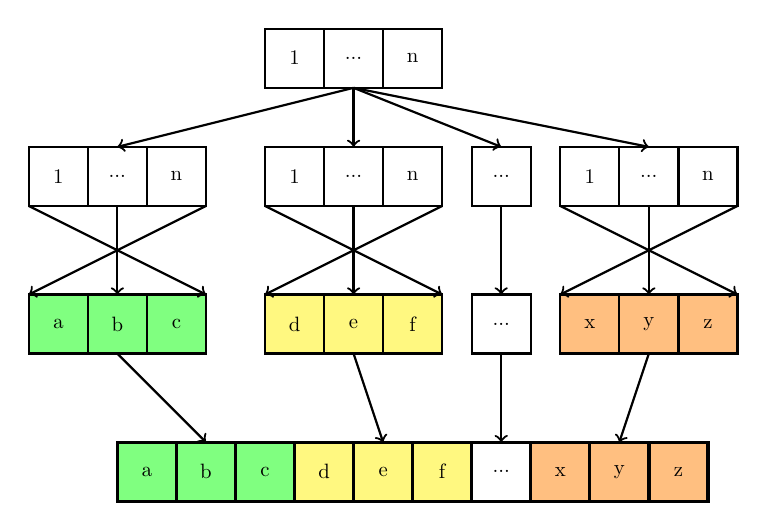
\begin{tikzpicture}[scale=0.75, transform shape]
	\draw [thick] (1,6.5) rectangle(2,7.5) node[pos=.5]{1};
	\draw [thick] (2,6.5) rectangle(3,7.5) node[pos=.5]{...};
	\draw [thick] (3,6.5) rectangle(4,7.5)node[pos=.5]{n};
	
	\draw [thick] (-3,4.5) rectangle(-2,5.5)node[pos=.5] {1};
	\draw [thick] (-2,4.5) rectangle(-1,5.5)node[pos=.5] {...};
	\draw [thick] (-1,4.5) rectangle(0,5.5)node[pos=.5] {n};
	
	\draw [thick] (1,4.5) rectangle(2,5.5)node[pos=.5] {1};
	\draw [thick] (2,4.5) rectangle(3,5.5)node[pos=.5] {...};
	\draw [thick] (3,4.5) rectangle(4,5.5)node[pos=.5] {n};
	
	\draw [thick] (4.5,4.5) rectangle(5.5,5.5)node[pos=.5] {...};
	
	\draw [thick,] (6,4.5) rectangle(7,5.5)node[pos=.5] {1};
	\draw [thick] (7,4.5) rectangle(8,5.5)node[pos=.5] {...};
	\draw [thick] (8,4.5) rectangle(9,5.5)node[pos=.5] {n};
	
	
	\draw [thick, fill=green!50] (-3,2) rectangle(-2,3)node[pos=.5] {a};
	\draw [thick, fill=green!50] (-2,2) rectangle(-1,3)node[pos=.5] {b};
	\draw [thick, fill=green!50] (-1,2) rectangle(0,3)node[pos=.5] {c};
	
	\draw [thick, fill=yellow!50] (1,2) rectangle(2,3)node[pos=.5] {d};
	\draw [thick, fill=yellow!50] (2,2) rectangle(3,3)node[pos=.5] {e};
	\draw [thick, fill=yellow!50] (3,2) rectangle(4,3)node[pos=.5] {f};
	
	
	\draw [thick] (4.5,2) rectangle(5.5,3)node[pos=.5] {...};
	
	\draw [thick, fill=orange!50] (6,2) rectangle(7,3)node[pos=.5] {x};
	\draw [thick, fill=orange!50] (7,2) rectangle(8,3)node[pos=.5] {y};
	\draw [thick, fill=orange!50] (8,2) rectangle(9,3)node[pos=.5] {z};

	
	\draw [very thick, fill=green!50] (-1.5,-0.5) rectangle(-0.5,0.5)node[pos=.5] {a};
	\draw [very thick, fill=green!50] (-0.5,-0.5) rectangle(0.5,0.5)node[pos=.5] {b};
	\draw [ very thick, fill=green!50] (0.5,-0.5) rectangle(1.5,0.5)node[pos=.5] {c};
	\draw [ very thick, fill=yellow!50] (1.5,-0.5) rectangle(2.5,0.5)node[pos=.5] {d};
	\draw [very thick, fill=yellow!50] (2.5,-0.5) rectangle(3.5,0.5)node[pos=.5] {e};
	\draw [very thick, fill=yellow!50] (3.5,-0.5) rectangle(4.5,0.5)node[pos=.5] {f};
	\draw [ very thick] (4.5,-0.5) rectangle(5.5,0.5)node[pos=.5] {...};
	\draw [ very thick, fill=orange!50] (5.5,-0.5) rectangle(6.5,0.5)node[pos=.5] {x};
	\draw [ very thick, fill=orange!50] (6.5,-0.5) rectangle(7.5,0.5)node[pos=.5] {y};
	\draw [ very thick, fill=orange!50] (7.5,-0.5) rectangle(8.5,0.5)node[pos=.5] {z};
	
	\draw [thick,draw=black,->] (2.5,6.5) -- (-1.5,5.5);
	\draw [thick,draw=black,->] (2.5,6.5) -- (2.5,5.5);
	\draw [thick,draw=black,->] (2.5,6.5) -- (5,5.5);
	\draw [thick,draw=black,->] (2.5,6.5) -- (7.5,5.5);
	
	\draw [thick,draw=black,->] (-3,4.5) -- (0,3);
	\draw [thick,draw=black,->] (-1.5,4.5) -- (-1.5,3);
	\draw [thick,draw=black,->] (0,4.5) -- (-3,3);
	
	\draw [thick,draw=black,->] (1,4.5) -- (4,3);
	\draw [thick,draw=black,->] (2.5,4.5) -- (2.5,3);
	\draw [thick,draw=black,->] (4,4.5) -- (1,3);
	
	\draw [thick,draw=black,->] (5,4.5) -- (5,3);
	
	\draw [thick,draw=black,->] (6,4.5) -- (9,3);
	\draw [thick,draw=black,->] (7.5,4.5) -- (7.5,3);
	\draw [thick,draw=black,->] (9,4.5) -- (6,3);
	
	\draw [thick,draw=black,->] (-1.5,2) -- (0,0.5);
	\draw [thick,draw=black,->] (2.5,2) -- (3,0.5);
	\draw [thick,draw=black,->] (5,2) -- (5,0.5);
	\draw [thick,draw=black,->] (7.5,2) -- (7,0.5);
	

	\end{tikzpicture}
	\caption[3.Optimierungsschritt]{Darstellung des dritten Optimierungsschritts. Hier werden die einzelnen Schritte des Ausgangsarray bis zum sortierten Array dargestellt.Der Master fügt die sortieren Teilarrays am Ende zusammen.}
	\label{fig:Ooptimierung}
\end{figure}

%Mögliche Optimierung (wenn nicht gewünscht weglassen)
\subsection{Optimierter Algorithmus}
Zusätzlich zu den Optimierungen am bestehenden Algorithmus wird eine alternative Aufteilung und Sortierung der Daten erarbeitet. Anstatt den initialen Vektor von einem Master Knoten aus auf eine beliebige Anzahl Worker aufzuteilen, kann eine Baumstruktur erstellt werden. Dabei sendet ein Ursprungsknoten die Hälfte des Datensatzes an einen weiteren Knoten. Diesen Prozess setzt jeder Knoten unabhängig fort, bis alle Rechenknoten verwendet werden. Anschließend führt jeder Knoten die Sortierung durch und sendet den sortierten Vektor wieder an den Knoten zurück, von welchem der Vektor empfangen wurde. Dieser Knoten führt durch die bestehende Funktion des Merge-Sorts die beiden sortierten Vektoren in einen sortierten Vektor zusammen und sendet diesen wiederum an den nächsthöheren Knoten. Dieser Prozess wird wiederholt, bis der Urpsrungsknoten die gesamten Daten hat. Das Ergebnis ist ein sortierter Vektor. Es werden hierbei nicht nur die Sortierungen Parallelisiert, sondern auch das Versenden sowie das Zusammenführen der Daten. Die gleichzeitige Ausführung von mehreren Prozessen sorgt dabei für eine bessere Ausnutzung der verfügbaren Rechenkapazitäten. Aufgrund von begrenzter Projektzeit wird dieser Algorithmus im Rahmen dieser Arbeit nicht implementiert oder getestet.
\begin{figure}[!t]
	\centering
	\includegraphics[width=3.5in]{Parallelisierungs_Algorithmus_2.png}
	\caption{Beispielhafter Durchlauf des Algorithmus mit 5 Nodes}
	\label{para_algo2}
\end{figure}
\section{Auswertung}
Die Autoren erwarten von ideal implementierter Parallelisierung einen messbaren Zusammenhang zwischen der Anzahl der verwendeten Rechenknoten und der resultierenden Laufzeit.
\\
Die im Abschnitt Ergebnisse durchgeführten Messungen lassen darauf schließen, dass Parallelisierung in der für das Projekt durchgeführten Form eine signifikante Absenkung der Laufzeit von bis zu einer Größenordnung von 60\% ermöglicht. Dieser Effekt ist jedoch stark begrenzt und flacht mit einer steigenden Rechenknotenanzahl schnell ab bzw. verschwindet gänzlich. Die Effizienz pro Rechenknoten nimmt daher bei steigender Anzahl von Rechenknoten ab. Für genauere Aussagen ist eine größere Anzahl an Messungen pro Messklasse für nötig.
\\
Eine Deutung für die beobachteten Ergebnisse: die Rechenknoten in der Cloud sind mittels Ethernet miteinander verbunden, was das Senden und Empfangen von Nachrichten erstens nicht zeitlich deterministisch und zweitens anfällig für unregelmäßige und längere Laufzeiten macht. Offenbar bewegt sich bei der kleineren Dateigröße das Senden und Empfangen von Nachrichten an mehr Knoten ab einer Knotenzahl von ca. vier in einer ähnlichen Größenordnungen wie der Laufzeitgewinn, welcher dadurch entsteht, dass ein Rechenknoten nur eine geringere Anzahl an Arbeit (Wörter sortieren) hat. 
\\
Es wird die These aufgestellt, dass bei einer größeren Datei mit mehr Wörtern ein Laufzeitgewinn auch bei größeren Knotenzahlen zu messen sein ist.
Um diese These zu untersuchen, werden die Ergebnisse der Messungen mit beiden Dateigrößen untersucht. Wie in IV. Ergebnisse erläutert verschiebt sich die Knotenzahl, ab der keine weitere Zeitreduktion zu messen ist, mit der größeren Datei von vier auf fünf. Dies widerlegt die Antithese, dass mehr Rechenaufwand sich \textit{nicht} auf den Auftretenszeitpunkt dieses Effektes auswirkt und untermauert die aufgestellte These.
\\
Während bei der kleineren Datei sich die Laufzeiten bei ausreichender Knotenzahl im Bereich von $1.6\text{s}$ einpendeln, werden bei doppelter Wörteranzahl etwa $5\text{s}$ benötigt. Der zugrunde liegende Merge Sort Algorithmus ist Teil der Komplexitätsklasse ${\mathcal{O}(n\log{n})}$. Es ist damit zu erwarten, dass die Laufzeiten bei gleicher Knotenzahl sich mehr als verdoppeln, also überlinear steigen. Dies wird durch die Mittelwerte für beide Dateigrößen in Tabelle 1 bestätigt. Bei gleicher Knotenzahl benötigt die Datei mit doppelter Länge bei jeder Knotenzahl mehr als die doppelte Laufzeit verglichen zur kleineren Dateigröße.
\\
Es wird die These untersucht, dass mit mehr Knoten die größere Wörteranzahl (und damit ein größerer Arbeitsaufwand) durch Parallelisierung kompensiert wird. Die Anzahl der Wörter, welche jeder Knoten im Fall \textit{kleine Datei, 3 Rechenknoten} und im Fall \textit{große Datei, 6 Rechenknoten} zu sortieren hat, ist identisch. Die benötigten mittleren Zeiten, $~2\text{s}$ vs.$~6\text{s}$ unterscheiden sich signifikant und widerlegen die These. Die Autoren vermuten die Funktion \textit{merge\_back()} als primäre und den erhöhten Sende- und Empfangsaufwand als sekundäre Erklärung hierfür. Grund hierfür ist, dass die Funktion \textit{merge\_back()} allein auf dem Master Knoten läuft. Entsprechend werden hier die Vorteile der Parallelisierung nicht genutzt. Bei Betrachtung von \textit{merge\_back()} ist zudem zu erkennen, dass die Laufzeit der Funktion von der Größe der zu sortierenden, vorsortierten Einzelelemente abhängt. Bei doppelter Wörterzahl sind doppelt so viele vorsortierte Wörtergruppen zu sortieren. Daher wäre aus Sicht der Autoren eine Erweiterung Funktion \textit{merge\_back()} um eine Parallelisierungsstrategie ein Angriffspunkt, um das Programm für große Wörterzahlen weiter zu optimieren.
\section{Fazit}
%\label{section:Fazit}
Durch den Vergleich zwischen der Laufzeit des Merge-Sort-Algorithmen ohne MPI mit dem parallelisierten Merge-Sort-Algorithmen werden Erkenntnisse gesammelt. Die Frage, die sich stellt: Bietet eine Parallelisierung mit MPI deutlich mehr Vorteile bei einem Merge-Sort-Algorithmus?\\

Bei der ersten Implementation benötigt der Merge-Sort der eingelesenen Datei von der Laufzeit länger. Erst ab fünf Prozessen ist MPI bei der Implementierung gleich schnell.
Bei der Gesamtlaufzeit ist die Laufzeit der Programmierung der Sende- und Empfangsvorgängen relevant. Die Zeit für die Sortierung nimmt einen geringen Anteil der Gesamtlaufzeit ein.
Da die Ausgangsimplementierung die Chars der Wörter einzeln versendet, erzielt eine Optimierung mit weniger Sende- und Empfangsvorgänge eine deutlich verbesserte Laufzeit. Durch diese Optimierung der ersten Implementation sind zwei Prozesse deutlich schneller als die Ausgangssituation ohne MPI. \\
Anhand der Laufzeit Messung ist ein graphischer Verlauf einer Exponentialverteilung zu erkennen, was darauf schließen lässt, dass bei einer gewissen Anzahl an Prozessen die Laufzeit nur minimal abweicht und bei vielen Prozessen eine Laufzeitverbesserung nicht mehr stattfindet.\\
Eine weitere Erkenntnis ist, dass die Laufzeit bei gleichbleibenden Prozessen und Wörtern keinen deterministischen Vorgang aufweist. Denn bei jedem neuen Aufruf des Merge-Sorts mit MPI variierte die Laufzeit. Dieses Ereignis tritt durch die Nutzung einer Cloud auf.\\

Zeitlich konnte der Optimierungsschritt III nicht mehr umgesetzt werden. Jedoch kann davon ausgegangen werden, dass die Laufzeit durch die beschriebene Optimierung \ref{Optimierung3} zusätzlich noch verbessert werden kann.

Anhand der Erkenntnisse und der Laufzeitauswertung ist zu sagen, dass MPI bei dem Merge-Sort-Algorithmus eine gute Performance bietet und die Laufzeit durch die Parallelisierung verkürzt. Das ist bei vielen Datenmengen mit umfangreichen Rechenanteil nützlich, damit die Prozesse parallel berechnet und die Ergebnisse am Ende zusammengeführt werden können.

\section*{Acknowledgment}

The preferred spelling of the word ``acknowledgment'' in America is without 
an ``e'' after the ``g''. Avoid the stilted expression ``one of us (R. B. 
G.) thanks $\ldots$''. Instead, try ``R. B. G. thanks$\ldots$''. Put sponsor 
acknowledgments in the unnumbered footnote on the first page.


\begin{thebibliography}{00}
\bibitem{b1} Dietmar Fey \glqq Grid-Computing: Eine Basistechnologie für Computational Science\grqq{}, Springer Verlag Heidelberg, Berlin, Seite 99-117 ,2010
\end{thebibliography}

\end{document}
